\chapter{Tri par Selection}
\section{Fonctionnement de l'algorithme}
Le tri par sélection (ou tri par extraction) est un algorithme de tri par comparaison.
Le principe du tri par selection est de :
\begin{itemize}
  \item rechercher le plus petit élément du tableau, et l'échanger avec l'élément d'indice 0.
  \item rechercher le second plus petit élément du tableau, et l'échanger avec l'élément d'indice 1.
  \item continuer de cette façon jusqu'à ce que le tableau soit entièrement trié.
\end{itemize}
\begin{figure}[H]
    \centering
        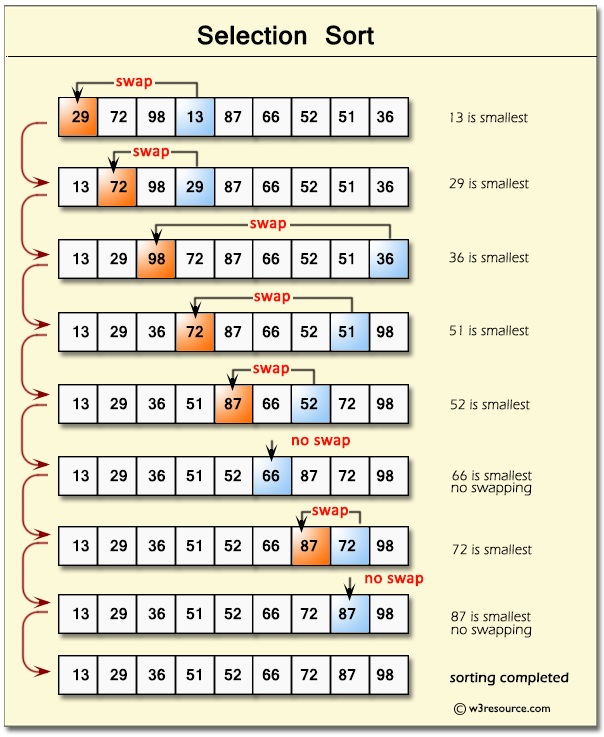
\includegraphics[scale=0.4]{ressources/selection-short.png}
        \caption{Exemple graphique d’un tri par selection}
    \label{fig:fusion}
\end{figure}
\par
Nous pouvons le représenter via le pseudo code suivant :
\par
\begin{function}[H]
    \textbf{Variables :}\\
    i,j : entier\;
    tmp,min : entier\;
    
    
    \Begin{
        \For{$i \leftarrow 1$ \KwTo N-1}{
            $min \leftarrow tab[i]$\;
            $j\leftarrow i$\;
            \For{$j \leftarrow i+1$ \KwTo N-1}{
            \uIf{tab[j] < tab[min]}{
                $min \leftarrow j$\;
               
            }
            }
            $tmp \leftarrow tab[min]$\;
            $tab[min] \leftarrow tab[i]$\;
            $tab[i] \leftarrow tmp$\;
        }
       
      
    }
    \caption{Selection(Entrée: tab: tableau d'entier; )}
\end{function}
\section{Calcul de complexité}
\subsection{Complexité temporelle}
Dans tous les cas, pour trier n éléments, le tri par sélection effectue au plus un nombre linéaire d'échanges :
\par
\textbf{Meilleur Cas:} 
aucun si l'entrée est déjà triée. 
\par
\textbf{Moyenne Cas:}
n-(1/2+...+1/n)= n-nln(n) c'est-à-dire si les éléments sont deux à deux distincts et que toutes leurs permutations sont équiprobables (en effet, l'espérance du nombre d'échanges à l'étape i est 
\par
\textbf{Pire cas:}
n-1 échanges qui est atteint par exemple lorsqu'on trie la séquence 2,3,…,n,1 ;
\par
Et donc le tri par sélection effectue \dfrac{n(n-1)}{2} comparaisons. Et sa complexité est donc O(n^2).
\par
le tableau suivant représente les temps d’exécution théorique en nanoseconde de l’algorithme selon la variation de la taille de l’expression :
\small
\begin{center}
\begin{tabular}{| c | c | c | c | c | c | c | c | c | c | c | c | c |}
    \hline
    N &  10 & 50 & 100 & 500 & 1000 & 5000 & 10000 & 100000 & 1000000 & 10000000 \\
    \hline
    t(ns) & 45 &
1225&
4950&
124750&
499500&
12497500&
49995000&
499995*10^4&
4999995*10^5&
49999995*10^6 \\
    \hline
\end{tabular}  
\end{center}
\par
La figure suivante représente l’évolution du temps d’exécution selon la longueur du tableau: 
\begin{figure}[H]
    \centering
        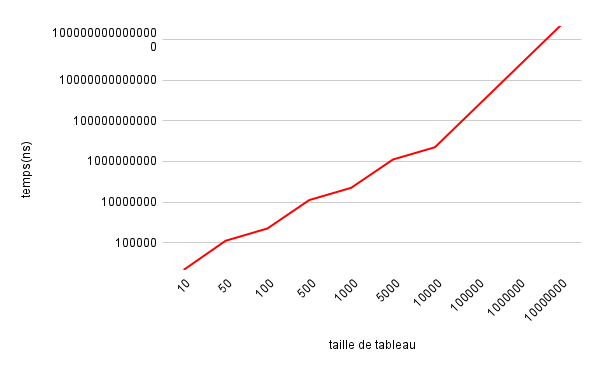
\includegraphics[scale=0.7]{ressources/chartselecttheorique.png}
        \caption{Temps d'exécution théorique du Tri Selection selon la longueur du tableau}
    \label{fig:temps_exec_selec_theo}
\end{figure} 
\subsection{Complexité spatiale}
Dans tous les cas O(1)
\section{Experimentation}
Le tableau suivant représente les temps d’exécution en nanoseconde de l’algorithme selon la variation de la taille et la configuration de l'entree .
\subsubsection{Les données du tableau sont triées en ordre inverse.}
\small
\begin{center}
\resizebox{19cm}{!}{
\begin{tabular}{| c | c | c | c | c | c | c | c | c | c | c |}
    \hline
    N &  10000 & 50000 & 100000 & 500000 & 1000000 & 5000000 & 10000000 & 50000000 \\
    \hline
    Temp(s) & 0.038229&
1.092237&
3.880469&
89.18019&
//&
//&//&//  \\
    \hline
\end{tabular}}
\end{center}
\normalsize
\subsubsection{Les données du tableau sont triées en bon ordre.}
\small
\begin{center}
\resizebox{19cm}{!}{
\begin{tabular}{| c | c | c | c | c | c | c | c | c | c | c |}
    \hline
    N &  10000 & 50000 & 100000 & 500000 & 1000000 & 5000000 & 10000000 & 50000000 \\
    \hline
    Temp(s) & 0.0324&
0.6452&
2.94&
78.785&//&//&
//&
//  \\
    \hline
\end{tabular}}
\end{center}
\normalsize
\par
\subsubsection{Les données du tableau sont aleatoires.}
\small
\begin{center}
\resizebox{19cm}{!}{
\begin{tabular}{| c | c | c | c | c | c | c | c | c | c | c |}
    \hline
    N &  10000 & 50000 & 100000 & 500000 & 1000000 & 5000000 & 10000000 & 50000000 \\
    \hline
    Temp(s) & 0.026639&
0.639662&
3.268848&
75.4&
//&
//&
//&
//  \\
    \hline
\end{tabular}}
\end{center}
\normalsize
\par
La figure suivante représente l’évolution du temps d’exécution en (s) selon la taille et la configuration du tableau :
\begin{figure}[H]
    \centering
        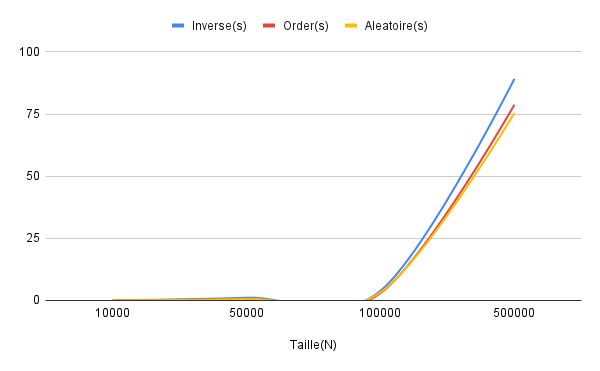
\includegraphics[scale=0.7]{ressources/selectexp.png}
        \caption{Temps d'exécution du programme selon la taille du tableau}
    \label{fig:temps_exec_dico_theo}
\end{figure} 
\par
Depuis le graphe, on observe que le temps d’exécution évolue de manière quadratique avec l’augmentation de la taille du tableau quelque soit la configuration utilise, ce qui correspond bien à la complexité théorique calculée auparavant.
\section{Conclusion}
L’algorithme de tri par selection se caractérise par son fonctionnement inconditionnel sur n’importe quel tableau. Par ailleurs, elle est coûteuse en temps. 